\documentclass[11pt, oneside]{article}   	% use "amsart" instead of "article" for AMSLaTeX format
\usepackage{geometry}                		% See geometry.pdf to learn the layout options. There are lots.
\geometry{letterpaper}                   		% ... or a4paper or a5paper or ... 
%\geometry{landscape}                		% Activate for rotated page geometry
%\usepackage[parfill]{parskip}    		% Activate to begin paragraphs with an empty line rather than an indent
\usepackage{graphicx}				% Use pdf, png, jpg, or eps§ with pdflatex; use eps in DVI mode
								% TeX will automatically convert eps --> pdf in pdflatex		
\usepackage{amssymb}

%SetFonts
\usepackage[T1]{fontenc}
\usepackage{lmodern}

%----macros begin-----------------------------------------------------------------------------------
\usepackage{graphicx}
\usepackage{color}

\def\conv{\mbox{\textrm{conv}\,}}
\def\aff{\mbox{\textrm{aff}\,}}
\def\B{\mathbb{B}}
\def\N{\mathbb{N}}
\def\E{\mathbb{E}}
\def\R{\mathbb{R}}
\def\Z{\mathbb{Z}}
\def\v#1{{\bf #1}}
\def\p#1{{\bf #1}}
\def\T#1{{\bf #1}}
\def\vet#1{{\left(\begin{array}{ccccccc}#1\end{array}\right)}}
\def\mat#1{{\left(\begin{array}{ccccccc}#1\end{array}\right)}}

\def\lin{\mbox{\rm lin}\,}
\def\aff{\mbox{\rm aff}\,}
\def\pos{\mbox{\rm pos}\,}
\def\cone{\mbox{\rm cone}\,}
\def\conv{\mbox{\rm conv}\,}

\newcommand{\floor}[1]{\left\lfloor #1 \right\rfloor}
\newcommand{\ceil}[1]{\left\lceil #1 \right\rceil}
%----macros end-----------------------------------------------------------------------------------


%SetFonts


\title{Fast algebraic filtering of surfaces from 3D medical images with Julia}
\author{Miroslav Ji\v{r}\'ik and Alberto Paoluzzi}
\date{}							% Activate to display a given date or no date

\begin{document}
\maketitle

\begin{abstract}
In this paper we introduce a novel algebraic \textsc{lar-surf} filter, well founded on algebraic topology methods, to extract and smooth the boundary surface of any subset of voxels arising from the segmentation of a 3D medical image. The input is defined as a \emph{chain}, i.e.~as a vector from a linear space of 3-chains, represented in coordinates as a sparse Boolean vector. The output is produced as the result of the mapping via the linear boundary operator $\partial_3:C_3 \to C_2$ between linear spaces of 3- and 2-chains.  In particular, when the input set of voxels is either not (4-)connected, or contains one or more empty regions inside, \textsc{lar-surf} generates a non connected set of closed surfaces, i.e.~a set of 2-cycles---using the language of algebraic topology. The only data structures used by this approach are sparse arrays with one or two indices, i.e.~sparse vectors and matrices. This work is based on LAR (Linear Algebraic Representation) methods, and is implemented in Julia language, natively supporting parallel computing on hybrid architectures.
\end{abstract}

\tableofcontents

%\section{}
%\subsection{}

\section{Introduction}\label{sec:intro}


Isosurface extraction to produce geometric models of surfaces from volumetric data is important in many applications. It is often used for indirect visualization of the medical data or for flow modeling \cite{Rohan2018a}. 
% In this paper we suggest an approach based on 
 
% Input volumetric data are represented by a 3D voxel field and can be generated by segmentation of sections from computed tomography. 
The most popular algorithm used for surface extraction is probably Marching Cubes (MC). The algorithm was described by Lorentsen and Cline \cite{Lorensen1987} in 1987. The survey of Marching Cubes algorithms has been published in 2006 \cite{Newman2006}. The algorithm is based on considering the cube defining volume. Each corner vertex of the cube is related to input volumetric data. MC traverse the data and constructs the surface by using a lookup table of different triangular faces depending on different patterns of the cube.  The main disadvantages of this method are time requirements, ambiguity, and holes generation. Some of them were discovered shortly after the algorithm was introduced. 
Marching Cubes. In 1991 Nielson and Hamman described an Asymptotic Decider to solve the ambiguity problem on the faces of the cube.  Natarajan noted that the ambiguity problem also occurs with uniform samples \cite{Natarajan1994}. In 1995 Chernyaev extended the number of cases to 33 \cite{chernyaev1995marching}. More recently the algorithm was updated by Custodio, Pesco, and Silva to enhance the quality of iso-surface triangulation \cite{Custodio2019}. 

Some alternative methods have been developed, including a method for surface extraction using particle attraction; a system was described by Crossno and Angel in \cite{Crossno1997}. A graph processing that tracks the boundary cell-face adjacencies is described in \cite{Lachaud2000}. Some parallel algorithms for iso-surface extraction are discussed in \cite{Bajaj2004}.
A completely data-parallel algorithm, implemented in OpenCL that runs entirely on the GPU is presented in~\cite{Smistad12}. 
A Linear Algebraic Representation approach, parallelized using the OpenCL framework on Linux, was discussed in~\cite{Paoluzzi2016}. % \cite{paodcvjcadanda2015}.

% In this paper
% TODO slightly change the formulation
Here we discuss an alternative approach for surface extraction. Our \textsc{lar-surf} (Linear Algebraic Representation Surface extraction) filter is based on basic algebraic topology and linear algebra, using linear spaces $C_p$ of chains (of cells) of dimension $0 \leq p \leq 3$ and the boundary matrix $[\partial_3] : C_3 \to C_2$.

Input volumetric data are represented by a 3D voxel array and can be generated by segmentation computed tomography (upper left image on Fig. \ref{fig:example_liver_macro_micro}). A decomposition of the input volumetric data into small submatrices called \emph{bricks} is performed, then the binary coordinate vector of each interesting chain of voxels is generated, and its boundary is computed by matrix multiplication times the boundary matrix producing the binary representation of the boundary surface (the surface which defines the boundary). 
Embarrassing parallel data decomposition is used to compute the boundary surface patches within each of the bricks, that are finally joined and smoothed via the Taubin algorithm \cite{Taubin1995}.

The present paper is organized as follows.
Section~\ref{sec:background} provides the basic topological and geometrical concepts needed to understand the \textsc{lar-surf} method, including the building of boundary matrices, the map from Cartesian indices to linear indices, and the Taubin smoothing method.
Section~\ref{sec:filter} discusses the parametric design of the unit block filtered by the parallel algorithm, including the block decomposition, the sparsity rate of the used sparse arrays, and the block-level parallelism.
Section~\ref{sec:julia} is related to the algorithm implementation in Julia, and in particular to a discussion of the parallel workflow.
Section~\ref{sec:examples} presents some examples of algorithm execution on the liver and the hepatic portal system.
Section~\ref{sec:conclusion} shortly describes the next extensions of this approach, in particular the implementation with Julia's support for GPU parallelism and the multi-segmentation of Medical images.


\section{Background}\label{sec:background}

Some basic concepts of solid modeling, and in particular the foundational idea of representation scheme, as well as few basic concepts of algebraic topology, are shortly introduced in this section, including the computation of the matrix of a boundary operator between chain spaces.

\subsection{Representation Scheme}\label{sec:schemes}

A \emph{representation scheme} for solid modeling is a mapping between a space of mathematical models and  space of symbolic representations like generated by a formal grammar.
Solid pointsets (i.e., `$r$-sets') are defined~\cite{Requicha:1980:RRS:356827.356833} as compact (bounded and closed) regular and semianalytic subsets of the $d$-space. A large number of representation schemes were defined in the past forty years, including the two main classes of (a) \emph{boundary representations} (`$B$-reps'), where the solid model is represented through a representation of its boundary elements, i.e.~faces, edges and vertices, and (b) \emph{decompositive/enumerative representations} \cite{Requicha:1980:RRS:356827.356833}, that are a decomposition of either the object or the embedding space, respectively, into a well-defined \emph{cellular complex}. In particular, a boundary representation provides a cellular decomposition of the object's boundary into \emph{cells} of dimension zero (vertices), one (edges), and two (faces). Medical imaging can be classified as the \emph{enumerative representation} of cellular decompositions of organs and tissues of interest \cite{Paoluzzi2016}, in particular, as subsets \emph{of 3D volume elements} (voxels) from the 3D image. 


\subsection{Linear Algebraic Representation}\label{sec:lar}


The \emph{Linear Algebraic Representation} (\textsc{lar}), introduced in~\cite{Dicarlo:2014:TNL:2543138.2543294}, aims to represent the \emph{chain complex}~\cite{TSAS,DiCarlo2009} generated by a piecewise-linear \emph{geometric complex} embedded either in 2D or in 3D. In a few words, it gets a minimal characterization of geometry and topology of a cellular complex, i.e.~the embedding mapping $\mu : C_0 \to \E^d$ of 0-cells (vertices), as well a description of $(d-1)$-cells as subsets of vertices, and is able to return the whole chain complex 
\begin{equation}
C_\bullet = (C_p, \partial_p) := 
C_3 
\substack{
\delta_2 \\
\longleftarrow \\
\longrightarrow \\
\partial_3 
}
C_2 
\substack{
\delta_1 \\
\longleftarrow \\
\longrightarrow \\
\partial_2 
}
C_1  
\substack{
\delta_0 \\
\longleftarrow  \\
\longrightarrow \\
\partial_1 
}
C_0 .
\end{equation}



%\[ 
%C_\bullet = (C_p, \partial_p) := 
%C_3 \ 
%\substack{
%\delta_2 \x
%\longleftarrow \[-1mm]
%\longrightarrow \
%\partial_3 
%}
%\ C_2 \ 
%\substack{
%\delta_1 \
%\longleftarrow \[-1mm]
%\longrightarrow \
%\partial_2 
%}
%\ C_1 \ 
%\substack{
%\delta_0 \
%\longleftarrow \[-1mm]
%\longrightarrow \
%\partial_1 
%}
%\ C_0 .
%\] 

% {   
%   \centering\vspace{1mm}
%   \includegraphics[width=0.475\textwidth]{figs/complex} 

% }

\noindent
and, in particular, any basis for linear chain spaces $C_p$, and any linear
boundary/coboundary map \(\partial_p\) and
\(\delta_p=\partial_{p-1}^\top\) between them. The \emph{domain} of \textsc{lar} is the set of \textbf{chain complexes} generated by cell $d$-complexes ($2\leq d\leq 3$). The computer \emph{representations} of \textsc{lar} are \textbf{sparse binary matrices} to represent both the operators and the chain bases. Note that in algebraic topology a $p$-chain is defined as a linear combination of $p$-cells with scalars from a field. When the scalar coefficients are from $\{-1, 0, +1\}$, a chain may represent \emph{any (oriented) subset of cells} from the cellular complex.
Scalars from $\{0, 1\}$ are used for non-oriented complexes.

We may, therefore, get the $(p-1)$-boundary $\partial_p c_p$ of \emph{any} $p$-chain $c_p$, by multiplication of the coordinate representation $[\partial_p]$ of the boundary operator times the coordinate representation $[c_p]$ of the chain in terms of such scalars, i.e.~by a  matrix-vector product $ [\partial_p] [c_p] $.

It is possible to show that the \textsc{lar} representation scheme is very expressive, i.e.~that it  has a large domain,  including collections of: line segments, quads, triangles, polygons, meshes;  pixels, voxels, volume images; B-reps, enumerative and decompositive representations of solids. 
In this paper we apply \textsc{lar} methods to computation of boundary representations of solid models from segmentation (labeling) of 3D medical images.
To display a triangulation of  boundary faces  in their proper position in space, the information required is contained in the \emph{geometric chain complex} (GCC):
\[
\mu: C_0\to\E^3,\ (\delta_0, \delta_1, \delta_2)
\qquad\equiv\qquad
\texttt{(geom, top) = (V, (EV, FE, CF))}
\]
The GCC allows to transform the (possibly non connected) boundary 2-cycle of surfaces as a standard B-rep~\cite{shapiroSM:202}. 
The geometry \texttt{geom} is given by
the embedding matrix \texttt{V} of vertices (0-cells), and  topology \texttt{top} by the three sparse matrices (\texttt{EV}, \texttt{FE}, \texttt{CF}) of coboundaries ($\delta_0, \delta_1, \delta_2$) of the chain complex describing a   
space arrangement~\cite{paoluzzi2019finite}.
Note that ordered pairs of letters from \texttt{V,E,F,C}, correspond to \emph{\emph{\texttt{V}}ertices$\to$\emph{\texttt{E}}dges$\to$\emph{\texttt{F}}aces$\to$\emph{\texttt{C}}ells} into the 
\emph{\emph{\texttt{C}}olumn$\to$\emph{\texttt{R}}ow} order of matrix maps of operators.



\subsubsection*{Construction of boundary matrix $\partial_d$}

First, let us fix an ordering for all the cells of a partition of input data (with vertices $V$, edges $E$, pixels $F$, and voxels $C$), i.e.~for each 0-, 1-, 2-, and 3-elements of a cell partition \texttt{V,E,F,C} of a 3D image, i.e., once fixed the $p$-bases for linear spaces $C_p$ of $p$-chains $(0\leq p\leq 3)$, we call $M_p = (m_{i,j})$ the \emph{characteristic matrix} of the $p$-basis, expressed as subsets so that 
$m_{i,j}=1$ if and only if the $j$-th  $0$-cell $c^j_0$ belongs 
% , where  we have that $m_{i,j}=1$ if and only if the $j$-th $0$-cell belongs 
to the boundary of $i$-th $p$-cell $m_{i,j}$, and $m_{i,j}=0$ otherwise.  

Let us note that the product of binary matrices is not binary, so by computing the (sparse) matrix product $(M_{p-1} M_{p}^t) = (n_{i,j})$, with $n_{i,j} = \sum_{k} m_{i,k}m_{k,j}$, we get for each $n_{ij}$ the \emph{number of vertices} shared by $c_{p-1}^i$ and $c_{p}^j$. When this number equates the cardinality of $c_{p-1}^i$, this elementary chain is contained on the boundary of $c_{p}^j$. In a volumetric data, with cubic 3-cells and squared 2-cells in-between, everywhere we get $n_{i,j}=4$, we may state $c_{2}^i\subset\partial c_{3}^j$. Therefore, in each $j$ column of $M_{2} M_{3}^t = (n_{i,j})$, we have exactly \emph{six rows} where  $n_{i,j} = 4$, since a cube (3-chain) has six boundary faces (2-chains). The unit incidence coefficients in $\left[\partial_3\right]$ are accordingly located by filtering the coefficients with value 4.

Finally, consider the linear graded boundary operator $\partial_p : C_p \to C_{p-1}$. As such, it contains by columns the representation of domain basis elements, expressed as a linear combination of the basis elements of the range space. Therefore, the operator matrix $[\partial_d]$ is readily obtained by setting $[\partial_d](i,j)=1$ if $n_{i,j}=4$ and $[\partial_d](i,j)=0$ otherwise.  Of course, it will contain six non-zero elements for the column.  It may be worth remembering every 3-cell (voxel) of the volumetric data has exactly six 2-faces. 

It is possible to show that all the interesting relations of incidence/adjacency between cells of different dimensions can be both computed and efficiently queried by pairwise computing some matrix products, with one of terms possibly transposed, using only the two boundary and coboundary operator matrices $[\partial_p]$ and $[\delta_p]$, and where $[\delta_p] = [\partial_p^\top]$. We~may also show that such matrices are \emph{very sparse}, with their sparseness growing rapidly with the dimensions (see Section~\ref{sec:brick}). The pattern of non-zeros in matrix $[\partial_3]$ corresponding to a brick of shape $(4,4,4)$ is given in Fig.~\ref{fig:boundary_matrix_4x4x4}.

\begin{figure}[tbp] %  figure placement: here, top, bottom, or page
   \centering
   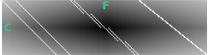
\includegraphics[width=0.75\linewidth]{src/figs/boundary_matrix_4x4x4_desc.png} 
   \caption{
   The binary image of \emph{sparse} coboundary matrix  $\left[\delta_2\right] = \left[\partial_3\right]^t : C_2 \to C_3$,
%   The binary image of the coboundary operator  $\delta_2 = \partial_3^\top : C_2 \to C_3$, 
   built for a small volumetric data (or a brick) with shape $(4,4,4)$. Note that the number of rows equates the size $4\times 4\times 4 = 64$ of the voxel set; the number of columns is $d\,n\,(1+n)^{d-1} = 3\times 4\times 25 = 300$. Of course, the number of non-zeros per row (cardinality of the facet set of a single voxel) is six, whereas the number of non-zeros per column is two, but on boundary facets.}
   \label{fig:boundary_matrix_4x4x4}
\end{figure}

\subsection{Multiindices from Cartesian indices}\label{sec:inds-from-cart}

In order to utilize the topological algebra shortly recalled in this paper, we need to explicitly sort the cells of the various dimensions into linearly ordered sequences, possibly according to the linear order their information is linearly accommodated in computer storage. 

\subsection{Taubin Smoothing}\label{sec:taubin}

Every boundary chain extracted from an image block $\B(i,j,k,n)$ is a \emph{2-cycle}, i.e., a closed 2-chain---in other words, a 2-chain with empty boundary. Such 2-cycles are joined together by removing the double 2-cells (at the boundaries of adjacent bricks) after having suitably shifted their indices to an unique linear representation of the whole image. The resulting raster surface is made by mutually orthogonal raster facets, that must be smoothed in order to get a fair surface. A linear time and space algorithm for this purpose is the Laplacian smoothing, which iteratively  moves each vertex (0-cell) to the centroid of its neighbors. A well known weakness of this simple algorithm is the asymptotic convergence of the whole mesh to a single point, resulting in unfair size reduction even after few iterations.  Conversely, the Taubin smoothing algorithm~\cite{Taubin:1995:SPA:218380.218473,egst.20001029} alternates two Laplacian smoothing steps with \emph{shrink} and \emph{inflate} effects respectively, with the result of delivering pretty invariant sizes and volume of the smoothed mesh. The best results are obtained on meshes which have small variations of edge length and face angles, like for surfaces extracted from 3D raster images, as in our case.
 


\section{Filter design and implementation}\label{sec:filter}



\subsection{Block-parametric design}\label{sec:block}

\subsubsection{Block decomposition}\label{sec:bbbb}

We assume that medical devices produce 3D images with lateral dimensions that are integer multiples of some powers of two, like 128, 256, 512, etc.
Any cuboidal portion of image is completely determined by the Cartesian indices of its voxel of lowest and highest indices, and denoted as $Image([\ell_x, \ell_y, \ell_z],[h_x, h_y, h_z])$.

For the sake of simplicity, we assume a common size on the three image axes, and the corresponding image portion $B$, called \emph{block}, as a function of its element of the  lowest  block  coordinates $i,j,k\in\N$ and of block dimension $n$:
\[
B(i,j,k,n) := Image([in,jn,kn],[i(n+1),j(n+1),k(n+1)]) 
\]

\begin{figure}[htbp] %  figure placement: here, top, bottom, or page
   \centering
   \includegraphics[width=2in]{figs/blocks} 
   \caption{A possible block partitioning of a radiologic image. The evidenced 2D block is $B([2,1,64]) = Image([128,64],[172,128)]$}
   \label{fig:blocks}
\end{figure}


Figure~\ref{fig:blocks} shows the block decomposition in a 2D case, with positive integer $u,v$ lateral sizes of image. Note that block sides do not necessarily correspond to image edges. 


\subsubsection{Block operator }\label{sec:bbbb}

\paragraph{Chain coordinates }\label{sec:bbbb} 
We are going to treat each image block independently from each other. Hence we map each image subspace $B(i,j,n)$ to the linear \emph{chain} space $C_2$ of dimension $n\times n$, using coordinate vectors $c_{h,k}\in \B^{n\times n} := \{0,1\}^{n\times n}$, where the basis element $c = c_{h,k} \in C_2$ is mapped via Cartesian-to-linear map to the Boolean vector 
\[
Image(h,k) \mapsto c_{h,k} := [0 \cdots 0\ 1\ 0 \cdots 0] \in \B^{n\times n}
\]
for each $0\leq h,k \leq n$, and where the (single) unit element is in position $nk + h \leq n\times n$.

Therefore, each pixel (or voxel) in a block image will be seen as a basis Boolean vector in $C_2$, and each subset of image elements, as the corresponding Boolean vector in $C_2$, with many ones as the cardinality of the subset.

\paragraph{Boundary operator }\label{sec:bbbb} For a fixed block size $n$, the boundary operator $\partial_d : C_d\to C_{d-1}$, with $d\in\{2,3\}$, will be constructed once and for all using the algorithm given in~\cite{}, and inlined in the generated boundary extraction code.

It is easy to see that the operator's matrix $[\partial_d]$ is \emph{very sparse}, since it contains $2\times d$ non-zero elements (ones) for each column (of length $n^d$), i.e.~4 ones and 6 ones for the 2D and 3D case, respectively. In fact the matrix of a linear operator between linear spaces contains by columns the basis element of the domain space, represented in the target space. In our case, the former is an image element (2-cube or 3-cube), represented as the chain of its boundary---i.e. either a 1-cycle of 4 edges, or  a 2-cycle of 6 faces, respectively.  

The number of rows of $[\partial_d]$ equates the dimension of the linear space $C_{d-1}$, i.e.~the number of $(d-1)$-cells---elementary $(d-1)$-chains---in the cellular partition of the image. To compute their number, we act in two steps. (a) First we map one-to-one the $n^d$ $d$-cells with $d$ adjacent $(d-1)$-cells, so getting $d\,n^d$ distinct basis elements of $C_{d-1}$. (b) Then we complete this bases by adjoining $n^{d-1}$ boundary elements for each of the $d$ dimensions of the image, so providing further $d\,n^{d-1}$ basis elements for $C_{d-1}$. The dimension of $C_{d-1}$, and therefore the number of rows of $[\partial_d]$ matrix is $d\,(n^{d-1}+n^{d}) = d\,n\,(1+n)^{d-1}$. The number of column equates the number of basis elements of $C_d$, i.e.~the number $n^d$ of block elements.

\paragraph{Sparsity and size of boundary matrix }\label{sec:bbbb} 

As we have seen, we have $2d$ non-zero elements for each column of $[\partial_d]$, so that their total number is $2d\,n^d$. The number of matrix element is $d\,n\,(1+n)^{d-1} \times n^d$, giving a ratio of 
\[
\frac{\mbox{non-zero\ elements}}{\mbox{total\ elements}} = 
\frac{2d\times n^d}{d\,n\,(1+n)^{d-1} \times n^d} =
\frac{2}{n+n^d}
\]
Using sparse matrices in CSC (Compressed Sparse Column) format we get a storage size:
\[
mem([\partial_d]_{n^d}) = 2\times \#\mbox{nzero} + \#\mbox{columns} = 2\times 2d\,n^d + n^d = (4d+1)n^d.
\]
In conclusion, for block size $n=64$, the matrix $[\partial_d]$ requires for 2D images $9\times 64^2=36,864$ memory elements, and for 3D images $13\times 64^3=3,407,872$ memory elements. Counting the bytes for the standard implementation of a sparse binary matrix (1 byte for values and 8 bytes for indices) we get $(18d+8)n^d$ bytes, giving $176$\,KB for 2D and $15.872$\,MB for 3D.

\subsubsection{Block boundary mapping}\label{sec:bbbb}

Here we refer directly to the 3D case.
Let us call \emph{segment} the bulk content $S$ of interest within the input 3D image of size $(u,v,w)$. We aim to compute the segment boundary $\partial_3 S$. 
First we set the size $n$ of the block, in order to decompose the input $Image(u,v,w)$ into a fair number 
\[
M = \ceil{u/n} \times \ceil{v/n} \times \ceil{w/n} = \frac{uvw}{n^3}
\] of blocks. 
Then we consider each image portion $c_{i,j,k} = S\cap B(i,j,k,n)$ and compute its (binary) coordinate representation  $[c]_{i,j,k}\in C_3(n,n,n)$. This one is a sparse binary vector of length $n^3$. Then assemble the $M$ representations $c$ of segment portions into a sparse binary matrix $\T{S}$, of dimension $n^d \times M$. Finally compute a matrix $\T{B}$ of boundary portions of $S$, represented by columns as chain coordinate vectors in $C_2$:
\[
\T{B} = [\partial_3(n)]\, \T{S}.
\]
where the boundary matrix has dimension $d\,n\,(1+n)^{d-1} \times n^d$.
Of course, the $\T{B}$ sparse matrix has the same column number $M$ of $\T{S}$, because each column contains the boundary representation of the corresponding $S\cap Box_{i,j,k}{i,j,k}$, and the number of rows of the operator, equal to the dimension of the linear space $C_2$.

\paragraph{Embedding}
A final computational step is needed, in order to embed the 2-chains in Euclidean space $\E^3$ and to assemble the whole resulting surface. In particular, we need to compute the \emph{embedding function} $\mu : C_0 \to \E^3$, where $C_0$ is the space of 0-chains, one-to-one corresponding to the vertices of the extracted surface. The simplest solution is to associate  four 0-cells to each 2-cell of the extracted surface, i.e.~to each non-zero entry in every column of \T{B}.  The $\mu$ function  can be computed by identifying, via  element position in the column, a triple of integer values $0\leq x\leq u$, $0\leq y\leq v$, and $0\leq z\leq w$ for each vertex of the 2-cell.  The mapping can be implemented using a dictionary, that will store the inverse coordinate transformation used at the beginning, i.e.~the one from linear to Cartesian coords, in order of not duplicating the output vertices.   

\paragraph{Surface assembling}

All boundary surface subsets $B_{i,j,k}(S) = \partial_3 S \cap \mbox{Box}_{i,j,k}$, provided by  columns of $\T{S}$, are embedded in the same coordinate space. In formal terms: 
\[
\texttt{Lar}(S) := (\texttt{Geom}(S), \texttt{Top}(S)) = (\texttt{V}, \texttt{CV}),
\]
where, with respect to the \emph{chain complex} $C_3\to C_2\to C_1\to C_0$ induced by the input image $Im$ and segment $S_{i,j,k}$, we get
\begin{align}
\texttt{Geom} &:= \mu(C_0(_{i,j,k})) = \texttt{V},
\\
\texttt{Top} &:= C_3(S) = \T{S} \mapsto \texttt{CV}.
\end{align}
and
\begin{align}
\texttt{Lar}(B_{i,j,k}) &:= (\texttt{Geom}, \texttt{Top}) = (\texttt{W}, \texttt{FW}),
\\
\texttt{Geom} &:= \mu(C_0(B_{i,j,k})) = \texttt{W} \subset \texttt{V},
\\
\texttt{Top} &:= C_2(B_{i,j,k}) = \T{B}_{i,j,k} \mapsto \texttt{FW} \subset \texttt{FV}.
\end{align}


A translation transformation applied to each vertex subset $\texttt{W}_{i,j,k}$ with translation  vector $\v{t} = [i,j,k]$ will therefore move it in the final space position, so finally giving
\[
\texttt{Lar}(B) = \oplus_{i,j,k}\texttt{Lar}(\partial_3 S_{i,j,k})) = \oplus_{i,j,k}(\texttt{W}, \texttt{FW}) .
\]


\subsubsection{Block-level parallelism}\label{sec:bbbb}

In the computational pipeline introduced in this paper, several steps can be efficiently performed in parallel at image-block level, depending on the embarassingly data parallel nature of the problem. In particular, little effort is needed to separate the problem into a number of parallel tasks $S_{i,j,k}$, using multiarray slicing. The granularity of parallelism, depending on the block size $n$, is further enforced by the computation of a single boundary matrix $[\partial_d(n)]$, in turn depending on $n$, so that the initial communication cost of broadcasting the matrix to nodes can be carefully controlled, and finely tuned depending on the system architecture. The whole approach is appropriate  for SIMD hybrid architectures of CPUs and GPUs, since only the initial block setup of boundary matrix and image slices, as well the final collection of computed surface portions, require inter-process communication.









\subsection{Julia implementation}\label{sec:implementation}


\subsection{Code optimization}\label{sec:optimization}


\subsection{Performance analysis}\label{sec:analysis}


\section{Examples}\label{sec:examples}


The 
For an experiments the we used the dataset Ircad1b. 

\begin{table}
\begin{tabular}{rrrrrr}
\toprule
 ID &  z-resolution [mm] &  xy-resolution [mm] &  obj. voxels &  size xy &  size z \\
\midrule
  1 &               1.60 &            0.570000 &      2865131 &      512 &     129 \\
  2 &               1.60 &            0.782000 &      1648024 &      512 &     172 \\
  3 &               1.25 &            0.625000 &      2375079 &      512 &     200 \\
  4 &               2.00 &            0.742188 &      1132427 &      512 &      91 \\
  5 &               1.60 &            0.782000 &      2124505 &      512 &     139 \\
  6 &               1.60 &            0.782000 &      1828493 &      512 &     135 \\
  7 &               1.60 &            0.782000 &      1461944 &      512 &     151 \\
  8 &               1.60 &            0.561000 &      3215090 &      512 &     124 \\
  9 &               2.00 &            0.873047 &      1265420 &      512 &     111 \\
 10 &               1.60 &            0.736000 &      1871804 &      512 &     122 \\
 11 &               1.60 &            0.720000 &      1692716 &      512 &     132 \\
 12 &               1.00 &            0.679688 &      3341433 &      512 &     260 \\
 13 &               1.60 &            0.671000 &      2063109 &      512 &     122 \\
 14 &               1.60 &            0.720000 &      1633641 &      512 &     113 \\
 15 &               1.60 &            0.782000 &      1389572 &      512 &     125 \\
 16 &               1.60 &            0.698000 &      2717185 &      512 &     155 \\
 17 &               1.60 &            0.743000 &      2106497 &      512 &     119 \\
 18 &               2.50 &            0.742188 &      1220564 &      512 &      74 \\
 19 &               4.00 &            0.703125 &       583208 &      512 &     124 \\
 20 &               2.00 &            0.808594 &      1359697 &      512 &     225 \\
\bottomrule
\end{tabular}

\end{table}
\begin{table}
\begin{tabular}{lrrrrr}
\toprule
{} &  z-resolution [mm] &  xy-resolution [mm] &   obj. voxels &  size xy &      size z \\
\midrule
count &           20.00000 &           20.000000 &  2.000000e+01 &     20.0 &   20.000000 \\
mean  &            1.77750 &            0.725141 &  1.894777e+06 &    512.0 &  141.150000 \\
std   &            0.60273 &            0.077233 &  7.206126e+05 &      0.0 &   44.088756 \\
min   &            1.00000 &            0.561000 &  5.832080e+05 &    512.0 &   74.000000 \\
25\%   &            1.60000 &            0.693422 &  1.382103e+06 &    512.0 &  121.250000 \\
50\%   &            1.60000 &            0.739094 &  1.760604e+06 &    512.0 &  127.000000 \\
75\%   &            1.70000 &            0.782000 &  2.187148e+06 &    512.0 &  152.000000 \\
max   &            4.00000 &            0.873047 &  3.341433e+06 &    512.0 &  260.000000 \\
\bottomrule
\end{tabular}

\end{table}

\section{Conclusion}\label{sec:conclusion}

% In this paper we have introduced and discussed a Julia implementation of an algebraic filter to extract from medical 3D images the boundary sourface of a specific image segment, described as a 3-chain of voxels. We have shown a good advantage over standard marchin-cubes algorithms. Translations from cartesian indices of cells to linearized indices, and the sparse matrix-vector multiplication are the main computational kernels of this approach. The current implementation employs Julia's channels for multiprocessing, and can be extended to gain a much greater speed-up using hybrid architectures mixing  CPUs and GPUs of last generation. 

% % TODO from abstract
% We introduced a Julia implementation of an algebraic filter to extract from 3D medical images the
% boundary surface of some specific image segment, described as a 3-chain of voxels. Translations from
% Cartesian indices of cells to linearized indices, the computation of the sparse boundary matrices, and the
% sparse matrix-vector multiplication are the main computational kernels of this approach. We may show
% a good speed-up over marching-cubes algorithms. The existing implementation employs Julia's channels
% for multiprocessing. Currently, the computational pipeline is being strongly improved to gain a greater
% speed-up using native Julia implementation \texttt{CUDA.jl} of Nvidia programming platform 
% % TODO cite Besard2017 [7]
% , and the Julia's
% \texttt{SuiteSparseGraphBLAS.jl} framework 
% % TODO cite BULUK 2017 [8] 
% for graph algorithms with the language of linear algebra. In
% particular, we are extending its use pattern in order to work with general cellular complexes.


We introduced a Julia implementation of an algebraic filter to extract from 3D medical images the
boundary surface of some specific image segment, described as a 3-chain of voxels. Translations from
Cartesian indices of cells to linearized indices, the computation of the sparse boundary matrices, and the
sparse matrix-vector multiplication are the main computational kernels of this approach. 

The implementation of the \textsc{lar-surf} filter is available in the open-source repository and it can be installed using standard Julia package manager \cite{larsurf-github}.

% NEW next two sentences are new
We showed a good speed-up over marching-cubes algorithms. 
The existing implementation employs Julia's channels
for multiprocessing. 
Our performance experiment showed an optimal size of the brick size.
Parallelization makes a large portion of spared computational cost. 
%
Moreover, we expect additional improvement in the future because our approach is appropriate  for SIMD (Single Instruction, Multiple Data) hybrid architectures of CPUs and GPUs, since only the initial block setup of boundary matrix and image slices, as well the final collection of computed surface portions, require inter-process communication. 

\sloppy{
Currently, the computational pipeline is being strongly improved to gain a greater
speed-up using native Julia implementation \texttt{CUDA.jl} of Nvidia programming platform 
% TODO cite Besard2017 [7]
% \cite{Besard:2017}
\cite{Besard2019}
, and Julia's
\texttt{SuiteSparseGraphBLAS.jl} framework 
\cite{Buluc2017}
% TODO cite BULUK 2017 [8] 
for graph algorithms with the language of linear algebra. In
particular, we are extending its use pattern in order to work with general cellular complexes.
}



\end{document}  